\documentclass{standalone}
\usepackage{tikz}
\usepackage{amsmath, amssymb}
\usetikzlibrary{positioning}

\begin{document}

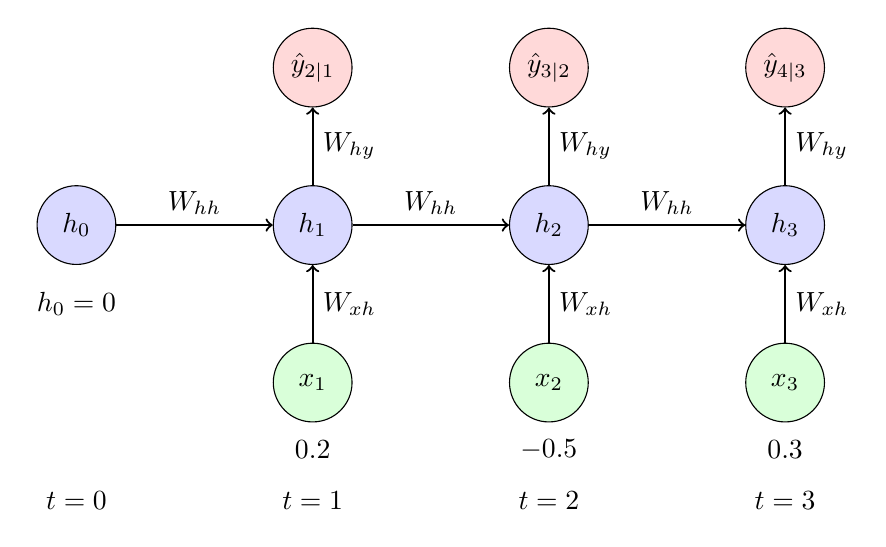
\begin{tikzpicture}[
          hidden/.style={circle, draw, minimum size=1cm, fill=blue!15},
          input/.style={circle, draw, minimum size=1cm, fill=green!15},
          output/.style={circle, draw, minimum size=1cm, fill=red!15},
          arrow/.style={->, thick}
        ]
          % hidden states
          \node[hidden] (h0) at (0,0) {$h_0$};
          \node[hidden] (h1) at (3,0) {$h_1$};
          \node[hidden] (h2) at (6,0) {$h_2$};
          \node[hidden] (h3) at (9,0) {$h_3$};

          % inputs with values
          \node[input] (x1) at (3,-2) {$x_1$};
          \node[input] (x2) at (6,-2) {$x_2$};
          \node[input] (x3) at (9,-2) {$x_3$};
          \node at (3,-2.85) {$0.2$};
          \node at (6,-2.85) {$-0.5$};
          \node at (9,-2.85) {$0.3$};

          % outputs: forecasts formed at origins t = 1, 2, 3 for dates t + 1
          \node[output] (y1) at (3,2) {$\hat{y}_{2\mid 1}$};
          \node[output] (y2) at (6,2) {$\hat{y}_{3\mid 2}$};
          \node[output] (y3) at (9,2) {$\hat{y}_{4\mid 3}$};

          % time labels
          \node at (0,-3.5) {$t=0$};
          \node at (3,-3.5) {$t=1$};
          \node at (6,-3.5) {$t=2$};
          \node at (9,-3.5) {$t=3$};

          % initial state annotation
          \node at (0,-1.0) {$h_0 = 0$};

          % recurrent arrows
          \draw[arrow] (h0) -- node[above] {$W_{hh}$} (h1);
          \draw[arrow] (h1) -- node[above] {$W_{hh}$} (h2);
          \draw[arrow] (h2) -- node[above] {$W_{hh}$} (h3);

          % input arrows
          \draw[arrow] (x1) -- node[right] {$W_{xh}$} (h1);
          \draw[arrow] (x2) -- node[right] {$W_{xh}$} (h2);
          \draw[arrow] (x3) -- node[right] {$W_{xh}$} (h3);

          % output arrows
          \draw[arrow] (h1) -- node[right] {$W_{hy}$} (y1);
          \draw[arrow] (h2) -- node[right] {$W_{hy}$} (y2);
          \draw[arrow] (h3) -- node[right] {$W_{hy}$} (y3);
\end{tikzpicture}

\end{document}
